\documentclass[instructions]{uqthesis}
% \usepackage{booktabs}
%\documentclass[final]{uqthesis} 


%*************************************
% FOR YOUR FINAL THESIS
%*************************************

%IMPORTANT! 
%The default document class (above - line 1 & 2) for the template is \documentclass[instructions]{uqthesis} - this document class will show instructional material and examples relevant to the preliminary material in the compiled PDF preview. THESE INSTRUCTIONS ARE FOR YOUR REFERENCE ONLY AND ARE NOT TO BE INCLUDED IN YOUR FINAL THESIS! 

%To turn off these instructions in your final thesis you MUST use the document class \documentclass[final]{uqthesis} 
%To activate the final thesis document class you must UN-COMMENT THIS DOCUMENT CLASS (remove the % from the start of line 2) and comment out the instructional document class on line 1 (add % to the start of line 1). 

%*************************************
% Introduction to template
%*************************************
%This is The University of Queensland Graduate School Official LaTeX Thesis template.

%Be sure to observe the content of comments within the source code, these are prefaced with a percentage symbol.
%Most important instructions have been CAPITALISED.
%To uncomment an inactive command (if required) remove the % from in front of the command.

%Please see the README for more information.

%This file loads the necessary packages, sets the page styles, and defines required macros.
%Edit this if you are comfortable with LaTeX.

%Other tweaks can be made in uqthesis.cls, but change these at your own risk!

%See README for version.

%You must have the memoir class installed.

% ***************************************************
% LaTeX Packages
% ***************************************************
% This file defines the document design.
% Usually it is not necessary to edit this file, but you can use it to change aspects of the design if you want.

%There are essential packages that are contained within the uqthesis.cls which are integral to the template - These must not be deleted.  A list of these packages can be found in the README.tet file

%The packages below are optional, please add or alter as required.

\usepackage{cite}				 %Allows abbreviated numerical citations.
\usepackage{pdfpages}			 %Allows you to include full-page pdfs.
\usepackage{wrapfig}			 %Lets you wrap text around figures.
\usepackage{bm} 				 %Bolded maths characters.
\usepackage{upgreek}			 %Upright Greek characters.
\usepackage{dsfont}				 %Double-struck fonts.
\usepackage{simplewick}			 %For typesetting Wick contractions.
\usepackage{mathtools}		     %Can be used to fine-tune the maths presentation.	
\usepackage{framed}			     %For boxed text.
\usepackage{microtype}			 %pdfLaTeX will fix your kerning.
\usepackage{marvosym}			 %Include symbols (like the Euro symbol, etc.).
\usepackage{color}				 %Nice for scalable pdf graphics using InkScape.
\usepackage{transparent}	     %Nice for scalable pdf graphics using InkScape.
\usepackage{placeins}			 %Lets you put in a \FloatBarrier to stop figures floating past this command.
\usepackage{mdframed,mdwlist}    %Use these for nice lists (less white space).
\usepackage{graphicx}            %Enhanced support for graphics.
\usepackage{float}               %Improved interface for floating objects. 
\usepackage{longtable}           %Allow tables to flow over page boundaries.
\usepackage{mathdots}            %Changed the basic LaTeX and plain TeX commands.
\usepackage{eucal}               %Font shape definitions to use the Euler script symbols in math mode.
\usepackage{array}               %Extending the array and tabular environments.
\usepackage{stmaryrd}            %The StMary’s Road symbol font.
\usepackage{amsthm}              %St Mary Road symbols for theoretical computer science. 
\usepackage{pifont}              %Access to PostScript standard Symbol and Dingbats fonts.
\usepackage{lipsum}              %Easy access to the Lorem Ipsum dummy text.
\usepackage{enumerate}           %Enumerate with redefinable labels. 
\usepackage[all]{xy}             %This is a special package for drawing diagrams.
\usepackage{amsmath}             %ATypesetting theorems (AMS style).
\usepackage{amssymb}             %Provided an extended symbol collection.
\usepackage[utf8]{inputenc}      %Allowed all displayable utf8 characters to be available as input.
\usepackage{fancyhdr}            %Extensive control of page headers and footers.
\usepackage{blindtext}           %Produced 'blind' text for testing.
\usepackage{tikz}                %To create graphic elements.
\usepackage[figuresright]{rotating}	%Allows large tables to be rotated to landscape.
\usepackage{makecell}
\usepackage{tabularx}
\usepackage{titlesec}


\usetikzlibrary{shapes.geometric, arrows}
%You can add more packages here if you need


%This defines some macros that implement Latin abbreviations
%COMMENT OUT OR DELETE IF UNDESIRED.
\newcommand{\via}{\textit{via}} %Italicised via.
\newcommand{\ie}{\textit{i.e.}} %Literally.
\newcommand{\eg}{\textit{e.g.}} %For example.
\newcommand{\etc}{\textit{etc.}} %So on...
\newcommand{\vv}{\textit{vice versa}} %And the other way around.
\newcommand{\viz}{\textit{viz}.} %Resulting in.
\newcommand{\cf}{\textit{cf}.} %See, or 'consistent with'.
\newcommand{\apr}{\textit{a priori}} %Before the fact.
\newcommand{\apo}{\textit{a posteriori}} %After the fact.
\newcommand{\vivo}{\textit{in vivo}} %In the flesh.
\newcommand{\situ}{\textit{in situ}} %On location.
\newcommand{\silico}{\textit{in silico}} %Simulation.
\newcommand{\vitro}{\textit{in vitro}} %In glass.
\newcommand{\vs}{\textit{versus}} %James \vs{} Pete.
\newcommand{\ala}{\textit{\`{a} la}} %In the manner of...
\newcommand{\apriori}{\textit{a priori}} %Before hand.
\newcommand{\etal}{\textit{et al.}} %And others, with correct punctuation.
\newcommand{\naive}{na\"\i{}ve} %Queen Amidala is young and \naive{}.

% ***************************************************
% Title page
% ***************************************************
%***THESIS TITLE***
%Use Sentence Case (capitalise only the first word and proper nouns).
\title{Image Detection with RISC-V Processor on FPGA}
\subtitle{Draft Project Proposal}

%***YOUR NAME***
%Do not include initials or middle names. Do not include your supervisor(s)' name(s).
\author{Joshua Wallace}
\studentnumber{45809978}
%***YOUR CURRENT DEGREES***
%Use abbreviations. Do not include the date or location of your degree. Do not include the degree for which this thesis is being submitted.
\currentdegrees{Project Proposal}

%***ORCID ID***
%Add and hyperlink your ORCID

%***YEAR OF SUBMISSION***
\date{2024}
%***TYPE OF DEGREE***
\submittedfor{Thesis - METR4911}


%***YOUR SCHOOL***
%Use Title Case (capitalise every word which is not a conjunction or preposition).
%See - http://blog.apastyle.org/apastyle/2012/03/title-case-and-sentence-case-capitalization-in-apa-style.html - for help.
\school{School of Information Technology and Electrical Engineering}

\begin{document}

\frontmatter
% Assemble title page
\maketitle
\clearpage

% ***************************************************
% Preface
%****************************************************
% \section{Abstract}
% \normalfont
% %Open abstract.tex to edit
% \input{./Abstract/Abstract.tex}

% \clearpage
% ***************************************************
% \section*{Declaration by author}
%DO NOT EDIT.
% \input{./Authordeclaration.tex}

\clearpage
%YOU MUST EDIT THIS DOCUMENT.
% ***************************************************
% PRELIMINARY PAGES
% ***************************************************
% The instructions contained within this part of the thesis template need to be suppressed from the final thesis. There are instructions on how to do this in the MainThesis.tex file.

% To ensure your work is not suppressed with the instructions please add your text only where instructed.


\clearpage
\pagestyle{headings}

\chapter[List of Abbreviations ]{List of Abbreviations}

%If the auto-sizing of the tables annoys you, consider the tabularx package.

%List of abbreviations.
\begin{center}
	\small
	\begin{longtable}{ll}
	\toprule
	Abbreviations & {} \\
	\bottomrule
	FPGA			& Field Programmable Gate Array \\
	ASIC			& Application Specific Integrated Circuit \\
	CPU				& Central Processing Unit \\
	GPU				& Graphical Processing Unit \\
	SoC				& System on Chip \\
	ISA				& Instruction Set Architecture \\
    RISC            & Reduced Instruction Set Computer \\
	CISC            & Complex Instruction Set Computer \\
	IO				& Input Output \\
	RTOS			& Real Time Operating System \\
	CNN			    & Convolutional Neural Network \\
    YOLO            & You Only Look Once \\
	VGA				& Video Graphics Array \\
	\hline 
	\end{longtable}
\end{center}

\clearpage

%***Table of Contents***
%These generate the table of contents, list of figures, and list of tables from items tagged with a \label{} command.
\tableofcontents
	\clearpage
\listoffigures
\listoftables

% \input{./PreliminaryAndBackPages/Symbols.tex} %List of symbols. REMOVE IF NOT NEEDED.

%***End of front matter***

% ***************************************************
% Thesis Content
%****************************************************
\mainmatter

%Each chapter is a separate .tex file. Use \input to load them here, as demonstrated below for Chapter 1 and Chapter 2.
%We recommend keeping each in a separate subfolder, with its accompanying figures, etc. This is how the template is currently structured.
%If you wish to divide your thesis into parts (each containing multiple chapters), us the \part{} command.

\chapter[Introduction]{Introduction}
\label{Chap:Intro}

\section{Introduction}

Introduction section

\chapter[Background]{Background}

\label{Chap:Background}

\section{Background}
A review of existing literature relevant to the topic has been conducted to provide a basis for the work. 
The related works to the research were selected: Field-Programmable Gate Arrays (FPGAs), RISC-V processors, image detection methods, and convolutional neural networks (CNNs). 
These are broadly discussed below, with a focus on the application of these technologies to image detection and hardware implementations.

\subsection{Image Detection and Analysis}
Image analysis is the process of extracting features from an image, to simplify it into a form that is more easily interpreted \cite{Mathworks}.
This often includes edge detection, object recognition, and image classification as subset actions.
Edge detection forms the basis of many image analysis techniques, as it is used to localize the variations in the image and to identify the physical phenomena which produce them \cite{Gradient}.
These are generally classed as gradient-based or Laplacian based, though gradient-based algorithms are dominant for the task \cite{Gradient}.

The Robert, Prewitt and Sobel techniques are the most prominent of the gradient-based algorithms, applying kernels to the image to detect edges \cite{Segmentation}.
\cite{XSG, Sobel, Canny, Aerial, Video} all provide a hardware implementation of the these filters, utilising the parallel processing capabilities of FPGAs to accelerate the gradient operations.
These designs realized improve efficiency in performance, per the throughput, and resource utilisation. 
Hence, FPGAs are providing a platform for processing real time algorithms on application-specific hardware with substantially higher performance than programmable digital signal processors (DSPs) \cite{RTEdge}.
This strongly indicates that FPGA-based implementations of image detection algorithms can offer significant improvements in running time for a range of digital signal processing methods.

The general pipeline for image detection and analysis is shown in Figure \ref{fig:pipeline}. This covers the available techniques which can be abstracted into hardware, to provide a high-speed, real-time image detection system.

\begin{figure}[h]
    \centering
    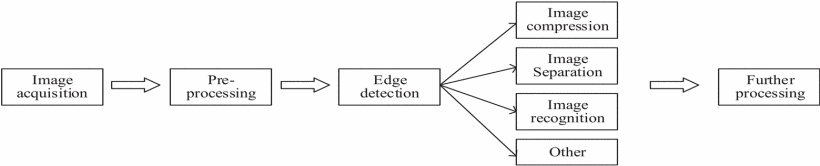
\includegraphics[width=1\textwidth]{Assets/Pipeline.png}
    \caption{Pipeline for image analysis techniques \cite{RTEdge}}
    \label{fig:pipeline}
\end{figure}

\cite{SoCImage, Aerial} follow a similar pipeline to Figure \ref{fig:pipeline}, with the image being captured by a camera module, and then processed by an FPGA though using differing image techniques.
The FPGA platform is optimal for any image detection tasks, as it can accelerate the required multiplication and addition operators separately - required for classical, and deep learning, based techniques \cite{ResourceEfficient}



\subsection{Convolutional Neural Networks and Deep Learning}
Convolutional neural networks (CNNs) are a type of artificial neural network that is primarily used for image detection.
Due to the lack of memory in low-end FPGA models, the CNN is optimal for an image processing task on SoC, as it has a low number of weights and biases relative to other neural networks \cite{Drowsiness}
The convolution operation requires a large number of multiply-accumulate (MAC) operations, and is the primary bottleneck in the performance of CNNs.
The operation must window over the entire image, and the number of MAC operations is proportional to the size of the image and the number of filters in the layer.
Hence, the CNN is computationally intensive, demanding a significant quantity of operations for high accuracy \cite{Linear}.
However, the proceeding \cite{Drowsiness} article found that the use of an embedded makes the implementation CNN less challenging on the FPGA platform, as the network can be designed in a systems language such as C.
This can then be compiled and translated into machine code, as there exists a toolchain for RISC-V.

Similar works for image-analysis using different neural network architectures have also been implemented using FPGA hardware.
\cite{Yolo, SparseYolo } demonstrates a hardware implementation of the You Only Look Once (YOLO) algorithm using a Xilinx Virtex-7 FPGA. 
Like the CNN hardware implementations, the architecture is focused on accelerating the convolution operation - and is a common denominator in the performance neural networks in hardware.
This acceleration is not specific to the convolution operator, and can be applied to any intensive operation in the network as the FPGA has little overhead on each operator when compared to traditional platforms \cite{Overhead}.
This is corroborated by \cite{Throughput}, which found that the implementation of hybrid neural networks on a Xilinix Virtex-7 690T FPGA achieved 4.13 times higher throughput than state of the accelerators in 2019.

\subsection{RISC-V}
Instruction set architectures (ISAs) define the operations a processor can execute, but the majority of ISAs are proprietary. 
Reduced Instruction Set Computing (RISC) is a form of ISA which offers a simpler, more efficient design than the traditional Complex Instruction Set Computing (CISC) ISAs - such as the prevalent x86 instruction set \cite{Arm}.
Arm and RISC-V are the two most prominent RISC ISAs, with Arm being the most widely used in embedded systems but with RISC-V offering royalty-free licensing and an open-source nature.
The lack of licensing fees and the open-source nature of RISC-V has led to its increasing popularity in the embedded systems domain \cite{Neutron}.
It is estimated that the number of chips utilising RISC-V technology "will grow 73.6 percent per year to 2027, when there will be some 25 billion AI chips produced, accounting for US \$291 billion in revenue" \cite{Drowsiness}.

There exists a number of FPGA implementations to create softcore processors using the RISC-V ISA \cite{RISCFPGA}. 
The 2023 paper \cite{Neutron} demonstrates a RISC-V implementation of the NEORV32 core, using a Wishbone bus interface. 
The authors selected the NEORV32 core due to the vendor-agnostic and platform independency, and the project being highly documented.
The softcore nature allows for the implementation details to be customised to the specific application, such that the core can be adapted to the specific use case \cite{DCT}. The NEORV32 processors offers a system-on-chip (SoC) Harvard architecture, with a 32-bit RISC-V processor, and a range of peripherals.
It supports UART, SPI, standard GPIO and the Wishbone b4 external bus interface for SoC connectivity \cite{NEORV32}.

As it is an open-source ISA, RISC-V has the added benefit of being extensible and modular \cite{Cryptography}, allowing for instructions to be added to the processor.
\cite{Reconfigurable} utilises this to create custom instructions within the RISC-V ISA to accelerate the expensive convolution operation for a CNN.

\subsection{Field-Programmable Gate Arrays}
Field Programmable gate arrays (FPGAs) provide flexible compute resources that can be reconfigured to suit a wide range of applications.
Similar to graphics processing units (GPUs), FPGAs offer parallel processing capabilities, but with the added benefit of reconfigurability \cite{Parallelism}.
The ability to develop custom logic designs is not unique to FPGAs, as application-specific integrated circuits (ASICs) also offer this capability, but FPGAs offer a faster development cycle and lower cost for low-volume production.
Hence, FPGA technology is optimal for edge applications on images due to the parallelised pipeline structure, which enables high-speed processing of large amounts of image data, and it's high processing speed ensures real-time image data processing \cite{Video}.

FPGAs have been studied extensively in the field of image detection, as replacements to existing hardware infrastructures. 
The most common application is to accelerate the convolution operation using the parallel processing capabilities of FPGAs. 

Figure \ref{fig:gradient} shows an implemention of a hardware-accelerated edge-detection algorithm for video images, using the Intel Cyclone IV FPGA platform direct from a camera module. 
This requires a camera module, FPGA and uses a VGA monitor to display the output - but does not use a softcore processor. 

\begin{figure}[h]
    \centering
    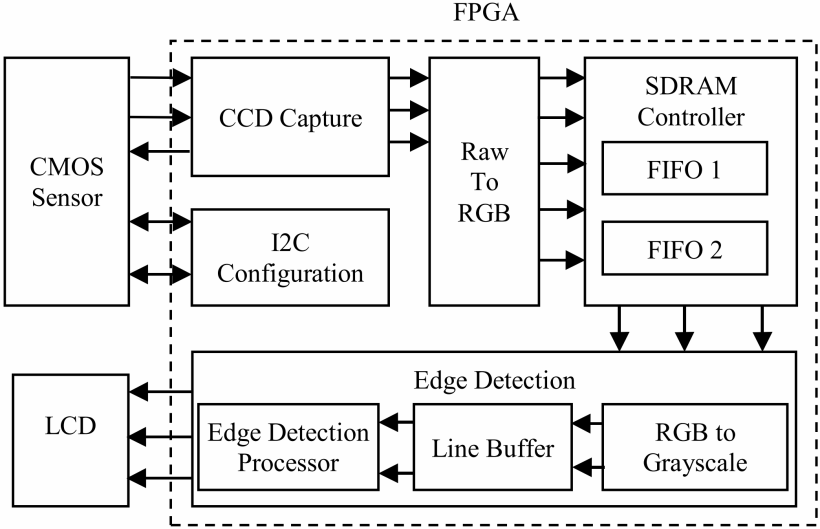
\includegraphics[width=1\textwidth]{Assets/Gradient.png}
    \caption{Video detection FPGA pipeline \cite{Gradient}}
    \label{fig:gradient}
\end{figure}

This pipeline has the core advantage over traditional CPU architectures which are serially structured, as it can perform the operations in hardware and in parallel. 
Hence, an image processing system employing an FPGA as the primary control chip is better suited to the low-latency and high speed demands of real-time image processing \cite{RTEdge}.

\chapter[Topic]{Topic}

\label{Chap:Topic}

\section{Topic}
Image detection, a critical task in computer vision, involves identifying and locating objects within images. 
Traditional software-based approaches for image detection often face challenges related to processing speed and resource utilization, particularly when dealing with large datasets or real-time applications. In response to these challenges, I propose leveraging Field-Programmable Gate Arrays (FPGAs) to accelerate image detection algorithms in hardware. By offloading computationally intensive tasks to FPGA-based hardware accelerators, we aim to significantly enhance the performance and efficiency of image detection systems.

The integration of FPGA-based hardware acceleration offers several compelling advantages. 
Firstly, FPGAs provide inherent parallelism and customizable hardware architectures, enabling efficient execution of image processing algorithms. 
This parallelism can lead to substantial improvements in processing speed, making real-time image detection feasible for applications such as surveillance, autonomous vehicles, and industrial automation. Additionally, FPGA-based solutions offer flexibility and scalability, allowing for the optimization of hardware resources to suit specific image detection requirements. 
This adaptability is particularly advantageous in scenarios where the detection algorithms need to be customized or updated frequently.

Furthermore, hardware-accelerated image detection using FPGAs can lead to significant reductions in power consumption compared to traditional CPU-based approaches, making it suitable for resource-constrained environments and embedded systems. 
By harnessing the computational efficiency of FPGA-based acceleration, we can achieve higher throughput and lower latency, thereby improving the responsiveness and effectiveness of image detection systems. 
Overall, this research aims to demonstrate the practical significance and utility of FPGA-based hardware acceleration in advancing the capabilities of image detection technology, paving the way for more efficient and scalable solutions in various domains.

Hence, this projects aim to:
\begin{itemize}
    \item Demonstrate the feasibility and benefits of FPGA-based hardware acceleration for image detection algorithms.
    \item Demonstrate the control of the image detection algorithm using a RISC-V softcore processor.
    \item Evaluate the performance, efficiency, and scalability of the FPGA-based image detection system.
\end{itemize}

It will not include the development of a new image detection algorithm or method, but rather the implementation of the algorithm in hardware, and the control of the algorithm using a RISC-V softcore processor.

\section{Overview}
The work can be divided into subcomponents to provide a timeline and structure to the project, as dependencies on previous work are required to progress.

\begin{figure}[h]
    \centering
    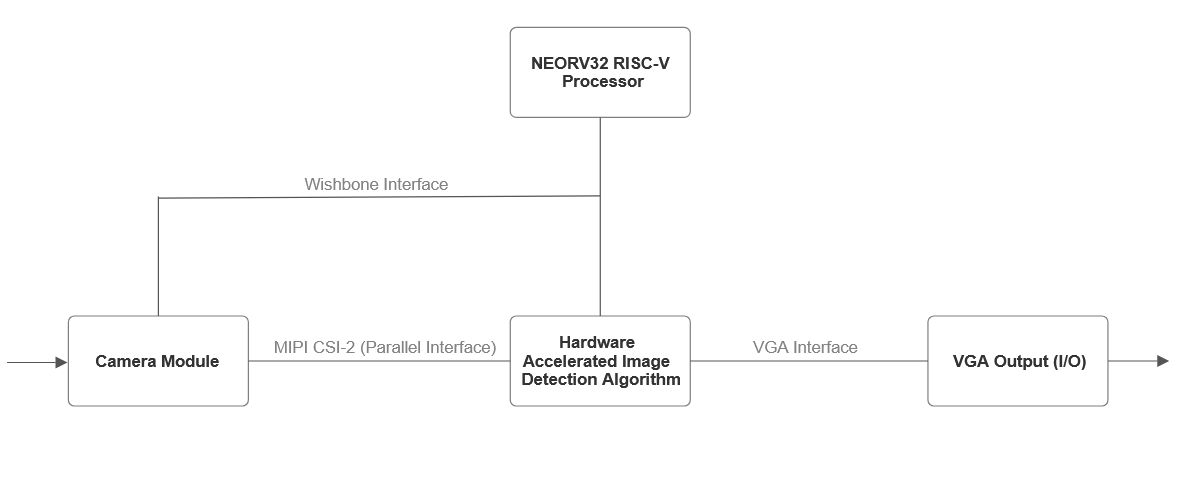
\includegraphics[width=1\textwidth]{Assets/Overview.png}
    \caption{Overview of proposed FPGA-based system.}
    \label{fig:overview}
\end{figure}

\subsection{Hardware}
The work will require the Xilinx Artix 7 XC7A100T FPGA, and a corresponding board to access I/O.
A Digilent Basys 3 board is available initially for development, however, a Digilent Nexys A7-100T board may be required depending on resource limits.
Both these boards use the Artix 7 XC7A100T FPGA, and have VGA outputs to allow for images to be displayed.
Figure REF below designates a high-level overview of the proposed system.

The camera module will be connected to the FPGA, and the NEORV32 processor will be used to control the image detection algorithm.

\subsection{Softcore Processor}
The NEORV32 RISC-V softcore processor has been selected due familiarity with it, and a highly documented ecosystem surrounding it. 
This processor will be implemented on the FPGA, and will be used to control the image detection algorithm, and display the processed image on a VGA monitor.

\subsection{Image Detection Algorithm}
The image detection algorithm has not yet been selected, and it is dependent on the resources available, and complexity desired.
The current options being considered are a convolutional neural network, such as in REF, or implementing classical imaging techniques via hardware such as that proposed in REF.
It is desired to implement a convolutional neural network, as image analysis is moving in the direction of deep learning algorithms \cite{DCNN}

\section{Performance Indicators}
The performance of the system to establish the success of the project are provided in Table \ref{tab:performance} below.


\begin{center}
    \small
    \begin{longtable}{lp{0.6\linewidth}}
        \label{tab:performance}
        \caption{Table of performance indicators.} \\
        \toprule
        Indicator & Description \\
        \midrule
        \endfirsthead
        
        \caption{Performance indicators to assess the success of the project. (continued)} \\
        \toprule
        Indicator & Description \\
        \midrule
        \endhead
        
        \bottomrule
        \multicolumn{2}{r}{\textit{Continued on next page}} \\
        \endfoot
        
        \bottomrule
        \endlastfoot
        
        Algorithm accuracy      & The ability of the system to correctly detect features in an image. \\
        Scalability             & A measure of the limits of the system in terms of image size, image complexity and algorithm complexity \\
        Throughput              & Measured as the number of images processed per time unit \\
        Latency                 & The time delay between acquisition of image and output of results relative to the clock-speed of the Xilinx Artix 7 XC7A100T FPGA \\
        Resource Utilization    & The amount of FPGA resources used to implement the system specified by number of LUTs and BRAM required for implementation \\
    \end{longtable}
\end{center}

\section{Required Resources}
The hardware will be designed using both a Digilent Basys 3 development board for initial prototyping, before being migrated to a Digilent Nexys A7-100T development board, to access more I/O and resources. 
Both boards have a VGA output, which will be used to display the processed image directly from the FPGA board. 
The specific camera module to be used has not yet been selected, however, a VGA OV7670 camera module which uses an I2C communication protocol is being considered for initial trials.
A VGA monitor will also be required to display the output of the processed image.

Benchmarking materials are dependent on the image detection algorithm selected, and cannot be provided at this time. Thus, the following resources are required for the project at this stage:

\begin{itemize}
    \item Xilinx Artix 7 XC7A100T FPGA
    \item Digilent Basys 3 FPGA Board
    \item Digilent Nexys A7 100T FPGA Board
    \item Camera Module
    \item VGA OV7670 Camera Module I2C
    \item VGA Monitor
    \item USB Power Supply
    \item VGA to VGA Cable
\end{itemize}

\chapter[Milestones]{Research Plan}

\label{Chap:Milestones}

\section{Milestones}
To track the development of the project, a set of milestones have been established with consideration of assessable dates. 
Table \ref{tab:milestones} below outlines the milestones for the work and what is required for each phase.
Emboldened text indicates an assessable milestone.


\begin{center}
    \small
    \begin{longtable}{p{0.25\linewidth}p{0.5\linewidth}p{0.15\linewidth}}
        \caption{Timeline of milestones.} \label{tab:milestones} \\
        \toprule
        Milestone & Description & Date \\
        \midrule
        \endfirsthead
        
        \caption{Timeline of milestones. (continued)} \\
        \toprule
        Milestone & Description & Date \\
        \midrule
        \endhead
        
        \bottomrule
        \multicolumn{3}{r}{\textit{Continued on next page}} \\
        \endfoot
        
        \bottomrule
        \endlastfoot
        
        \textbf{Project Proposal}	& Complete the project proposal and literature review.                                              & 23/4 \\
        Configure hardware			& Implement NEORV32 processor on FPGA, connect to external components through wishbone interface.   & 23/4 \\
        \textbf{Seminar}            & Present the current project status.                                                               & 23/4 \\
        Image detection algorithm   & Select and implement image detection algorithm in hardware.                                       & 23/4 \\
        VGA driver                  & Develop driver and interface to display processed image on VGA monitor.                           & 23/4 \\
        Benchmark                   & Benchmark system performance against related works.                                               & 23/4 \\
        \textbf{Demo}               & Demonstrate the complete project.                                                                 & 23/4 \\
        \textbf{Thesis}             & Document and write project results.                                                               & 23/4 \\
    \end{longtable}
\end{center}


\nopagebreak


\section{Risk Assessment}
This project is conducted in the low-risk laboratory covered by general OHS laboratory rules, and in a home setting. 
There are no hazardous materials or dangerous equipment used in the project, and the risk of injury is negligible.
The only risk to the project is hardware failure or proprietary software issues, which can be mitigated by using open-source software and hardware, and regular backups of the project files.
Redundancies are also in place for hardware failure, as two FPGA developments boards are designated for use.

% HOW TO ADD ADDITIONAL CHAPTERS
% Step One: Add a new folder called "ChapterX" (X being the chapter number).
% Step Two: Within the folder add a new .tex file by clicking the "New File" button in the Overleaf Menu. Rename the file to a title of your choice.
% Step Three: Copy the Chapter 2 headline and "\input" command located above and insert it below Chapter 2.
% Step Four: Rename the headline to your specific chapter number, change the input command to include the name of the folder you created and the name of the file you created.
% Repeat this process for every chapter.

%CONCLUSION CHAPTER
% \input{./Conclusion/Conclusion.tex}

% ***************************************************
% Bibliography
%****************************************************
%CHOOSE YOUR BIB STYLE AND FILE.
%We have included the following two referencing styles for you to use in your thesis. You can add an alternate style if you prefer.

%Style: apalike = this is an (Author, Year) referencing style similar to APA
%Style: elsarticle-num = this is a numbered referencing style that will display the bibliography in citation order

%To use one of the styles provided ensure the % is removed from the start of the line, and the other option is commented out with a % at the start of the line. The style elsarticle-num is active by default.

\bibliographystyle{ieeetr}

\bibliography{./References/Bibliography}

%When you have finished your thesis we recommend that you manually fix any errors in your bibliography. 
%To do this, compile, copy the .bbl into a new .tex file and include this here after commenting out the other bibliography commands. Make corrections in that .tex file.

% ***************************************************
% Appendices
%**************************************************** 
%UNCOMMENT THIS SECTION IF YOU ARE USING APPENDICES.
%Simply adapt the same formatting used for other chapters.
% \appendix
% If you need appendix in your thesis then consider the following appendix file (you can add more if you need more) otherwise you should not consider it in your main thesis.
% \include{./Appendix/Appendix}

% ***************************************************
% Examples
%**************************************************** 
% The following files are only for examples and you should not include them in your final thesis.
% \include{./Examples/ExampleOfCitations}
% \include{./Examples/ExampleOfCode}
% \include{./Examples/ExampleOfEquations}
% \include{./Examples/ExampleOfFigures}
% \include{./Examples/ExampleOfFlowCharts}
% \include{./Examples/ExampleOfTables}


% ***************************************************
% Back Matter
%**************************************************** 
% COMMENT OUT IF YOU DO NOT WISH TO INCLUDE BACK MATTER.
% \input{./PreliminaryAndBackPages/Back.tex}

\end{document}
